\section{Numerical study}
\label{sec:evaluation}
The published reference cases test the timing of repeated contact transitions and the geometry of a cam with prescribed motion. The continuous detection study compares general geometry queries on complete STEP boundaries. Appendix~\ref{sec:industrial} reports the mechanism-specific force integration experiments.

The C++ implementations use Release builds and binary64 arithmetic. The Windows STEP runs use MSVC and Open CASCADE 7.9.3 on an AMD Ryzen 9 5900X. We give setup and online integration time separately and exclude trace serialization. Cam setup includes common model preparation. The fixed-step cam comparison uses three runs for each support query and one for each general search. The selected spur and reducer timings use three and two serial runs, respectively. We report the median online time for repeated configurations. The Linux engine results were obtained on the same workstation under WSL. The RecurDyn timings report the Windows solver and process interface separately. Software versions, individual timing records and precise settings are in the repository.

\subsection{Unilateral spring oscillator}
\label{sec:oscillator}
We reproduce the unit-mass oscillator of Junca and Rousselet \citep[Sec.~2]{junca2009}. Its displacement obeys $\ddot u+\omega_0^2 u+\varepsilon[u]_+=0$, with $u(0)=a_0>0$ and $\dot u(0)=0$. We use the normalizations $\omega_0=1$ and $a_0=1$ and select $\varepsilon/\omega_0^2=0.1$ for the parameterized model. The oscillator spends $\pi/\sqrt{\omega_0^2+\varepsilon}$ time units in contact and $\pi/\omega_0$ detached per period. Matching the two harmonic solutions at $u=0$ gives the displacement and contact force $\varepsilon[u]_+$ throughout the run.

We integrate 50 periods with the HHT solver and evaluate the scalar spring law directly. Linear interpolation of the numerical displacement at neighboring steps gives the times of contact onset and release. Each run reproduces all 100 transitions. Table~\ref{tab:oscillator} shows the refinement results. At the finest step, the largest timing error over the run is $2.09\times10^{-4}$ time units. The maximum errors in the duration of complete contact and detached intervals are $2.15\times10^{-6}$ and $2.05\times10^{-6}$ time units, respectively. Figure~\ref{fig:oscillator} shows the displacement and the accumulated timing error. This case tests integration through repeated changes of contact state with an exact force callback.

\begin{table}[pos=!htbp]
\centering\small
\caption{Errors over 50 periods of the published unilateral spring model. RMS displacement and force errors and the maximum onset or release timing error use the normalized units of the reproduction.}
\label{tab:oscillator}
\begin{tabular}{lrrr}\toprule
Nominal step & RMS displacement error & RMS force error & Max. timing error \\\midrule
0.0100 & $1.44\times10^{-3}$ & $1.01\times10^{-4}$ & $3.35\times10^{-3}$ \\
0.0050 & $3.60\times10^{-4}$ & $2.52\times10^{-5}$ & $8.37\times10^{-4}$ \\
0.0025 & $9.01\times10^{-5}$ & $6.29\times10^{-6}$ & $2.09\times10^{-4}$ \\
\bottomrule\end{tabular}
\end{table}

\begin{figure}[pos=!htbp]
\centering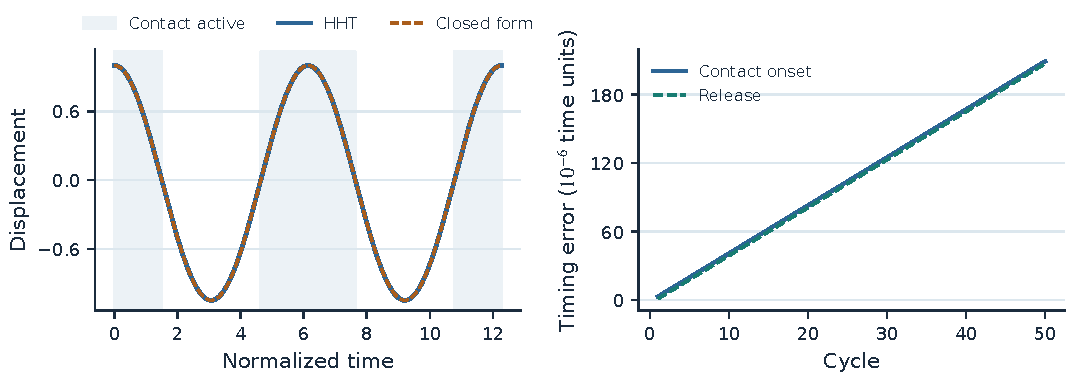
\includegraphics[width=.92\linewidth]{unilateral-response.pdf}
\caption{Unilateral oscillator with the finest HHT step. The first two periods show the motion and intervals of active contact. The onset and release timing errors are shown for all 50 periods.}
\label{fig:oscillator}
\end{figure}

\subsection{Constant-breadth cam and translating flat follower}
\label{sec:constant-breadth}
We reconstruct the Type I cam in Dhande and Rajaram's Example~1 \citep{dhande1984} from the six circular arcs of their Table~1. We use $a=6$, $b=5$, $c=7$, $d=2.5$, and $x_0=y_0=0$ in their length units. The cam rotates at $1$ rad/s between two parallel follower faces. Its constant breadth is $9$ length units. The guide and the opposing faces prescribe the follower translation. The reference comprises their displacement, velocity and acceleration equations over one complete revolution (Eqs.~(8), (10), and (12) and Table~2).

We rotate the reconstructed B-rep and obtain displacement from its supporting position along the follower translation axis. Position evaluation uses the CAD profile and its oriented extrema. Five-point finite differences at a spacing of $0.05^\circ$ yield velocity and acceleration. At the six arc junctions the acceleration changes discontinuously, so we report derivative errors at the 7,175 positions with stencils wholly inside an arc's contact interval. The maximum absolute CAD reconstruction errors are $2.66\times10^{-15}$ in displacement, $4.50\times10^{-12}$ in velocity and $1.31\times10^{-8}$ in acceleration, in the corresponding length and second units. Figure~\ref{fig:constant-breadth} shows the reconstructed motion and reference.

On the original $1^\circ$ sample grid we also import the CAD profile's extruded arc faces from STEP and use our bounded distance query to obtain a follower position interval at each pose. The 361 intervals, including both endpoints, contain the published position. The widest interval is $9.99\times10^{-5}$ length units and the maximum midpoint error is $4.91\times10^{-5}$ length units. This case verifies contact geometry and prescribed kinematics across all six profile sections.

\resultfigure{constant-breadth}{Reconstructed constant-breadth cam at $90^\circ$ between two translating flat faces, with an enlarged view of the contact on the right face. CAD kinematics and published solutions use the original length units and time in seconds. Acceleration curves are broken at the arc junctions.}{fig:constant-breadth}


\subsection{Continuous contact on complete CAD boundaries}
\label{sec:general-contact}
Our backend prepares each STEP boundary as trimmed patches and searches over the specified rigid motion. The tests use the same patch and trim operations for every shape. The axial-envelope shortcut and planar witness proposals are disabled. The mesh baselines use swept triangle prisms for translations and a triangle BVH distance query with a point-speed bound for rotation. We also test advancement with either bounded static B-rep distances or the independent numerical Open CASCADE distance kernel. For numerical distances the advancement uses a $10^{-6}$ mm margin. The numerical margin and mesh deflection do not give an outward enclosure of the nominal CAD surface.

\paragraph{Rotating cam with recorded contact transitions.}
We replay 22 accepted steps at contact onset from the eccentric-cam start-up and the immediately preceding step for each. Each replay keeps the recorded end poses and interpolates the angle and follower displacement within the step. The backends receive the two full STEP shapes and the rigid motion. The analytic cylinder--plane gap is evaluated separately at high precision to score the outcomes. The requested time width is $5\times10^{-4}$ of the 125~\microsec{} input step. The direct search and bounded static advancement each use a 20,000-task cap.

\begin{table}[pos=!htbp]
\small\centering
\caption{Rotating cam. An onset completes if its interval includes the reference time and meets the requested width. A preceding interval completes if it is reported inactive throughout. Query time is the median across all 44 paths after taking the median of two runs per path. It includes unresolved queries and excludes preparation.}
\label{tab:cam-onset}
\begin{tabular}{lrrr}\toprule
Method & Onsets (of 22) & Inactive (of 22) & Query (ms) \\\midrule
Direct B-rep interval search (ours) & 0 & 0 & 524.12 \\
Bounded B-rep distance + advancement & 0 & 0 & 300.76 \\
OCCT distance + advancement & 3 & 22 & 132.32 \\
Triangle BVH + advancement & 4 & 22 & 64.10 \\
\bottomrule\end{tabular}
\end{table}

Our search witnesses contact in three paths with brackets wider than the target and returns unresolved outcomes in the others. OCCT and the finest mesh report contact in all 22 onset paths. Most intervals are wider than the target. The mesh row uses a nominal deflection of 6.10 nm and requires 23.97 s of one-time mesh preparation. At 3.125~\micron{} deflection, 21 of the 22 onset paths disagree with the analytic reference. The data retain all six tessellation settings and the result of the mesh-guided CAD verification.

\paragraph{Production STEP assembly motions.}
We also run eight translation paths on the published OpenAMRobot MMP wheel and lidar assemblies and the Voron Trident Front Idler B assembly. All methods use the same original occurrences and path definitions. The requested bracket width is $5\times10^{-4}$ of the prescribed path duration, and B-rep search uses a 200,000-task cap. We compare the outputs with an adaptive numerical OCCT reference. This reference shares its distance kernel with the OCCT advancement baseline.

\begin{table}[pos=!htbp]
\small\centering
\caption{Production STEP translations. Completed results meet the requested width or exclude contact over the entire path and agree with the numerical reference. The reference remains unresolved on one of the eight paths. Online time is the median over all paths of three-run medians, excluding preparation.}
\label{tab:production-contact}
\begin{tabular}{lrr}\toprule
Method & Completed and compatible & Query (ms) \\\midrule
Direct B-rep interval search (ours) & 6 of 8 & 1034.05 \\
Bounded B-rep distance + advancement & 3 of 8 & 4609.70 \\
OCCT distance + advancement & 7 of 8 & 614.48 \\
Triangle BVH + swept-triangle CCD & 7 of 8 & 12.73 \\
Triangle CCD + bounded CAD advancement & 3 of 8 & 4814.83 \\
\bottomrule\end{tabular}
\end{table}

The mesh rows use the 3.125~\micron{} nominal deflection. The direct search completes the three wheel paths, the lidar pre-seat path and two idler paths. It retains a wider interval for full lidar insertion. The Voron spacer reference is unresolved, so that path contributes to the timing but has no success credit. The finest mesh and numerical OCCT methods agree with the reference on all seven resolved reference paths.


\paragraph{Loaded spur and reducer stages.}
We replay one 20~\microsec{} segment during the load rise for the spur pair and each reducer stage. Relative translation is interpolated between the recorded end poses in the driver frame. The deviations of these chords from the rotating center paths are bounded by 0.163~\micron{} under linear angular interpolation. The STEP boundaries are complete gear solids. Our search, OCCT advancement, and the finest tested triangle BVH report contact at the initial pose on all three segments. These checks exercise the same pipeline on involute and helical tooth surfaces under load. Each segment starts inside the contact layer, so this experiment has no onset time to localize within the step.

\paragraph{Chen et al.'s published patch example.}
We also run the official TDIB-CCD OBB solver \citep{chen2024} on its distributed \texttt{singleTest} case. Two orthogonal bicubic patches translate at the prescribed speeds. Their analytic intersection time is $10/17$ in the example's time units. The official implementation gives a candidate time of $0.5882353$ and a distance of $8.97\times10^{-4}$ between the returned parameter-cell centers. The median query time over five runs is 285.72 ms. The direct B-rep search proves the inactive interval up to $0.5882353$ and leaves the zero-distance witness unresolved at 25,000 tasks, with a median of 2,612.94 ms. This shared problem uses untrimmed patches and linear control-point motion. Matching the solver to the full STEP cases also requires trim-domain handling and an agreed model of rotating motion and contact activation.
\FloatBarrier

